%set the master document for easy compilation
%!TEX root = ../D3_5_3.tex

\section{F2.9: Manage\_Radio\_Communication and RBC\_Handover}\label{s:F2.9}

\subsection{Component Requirements}

\begin{longtable}{p{.25\textwidth}p{.7\textwidth}}
\toprule
Component name			& MoRC\_HO \\
\midrule
Link to SCADE model		& {\footnotesize \url{https://github.com/openETCS/modeling/tree/master/model/Scade/System/ObuFunctions/Radio/MoRC_HO}} \\
\midrule
SCADE designer			& Uwe Steinke, Siemens AG \\
\midrule
Description				&  

The \emph{MoRC\_HO} component implements the handover process between two different RBCs and the session management (\emph{MoRC} = management of radio communication) with each of them. 

MoRC\_HO comprises

\begin{itemize}
	\item the \emph{processHandingOver} subcomponent performing the handover process from the handing over RBC to the accepting RBC,
	\item two instances of \emph{MoRC\_Main\_v2} representing the session management with up to two RBCs in parallel
	\item a \emph{mobileDataRouter\_out} subcomponent for routing the OBUs output data stream to both RBCs and switching over from the handing over RBC to the accepting RBC. 
\end{itemize}

\emph{processHandingOver} consumes the relevant messages received from track and controls the registration with the radio network, the session termination with the handing over RBC and the session establishment with the accepting RBC. To achieve this, it controls up to two instances of \emph{MoRC\_Main\_v2}. Additionally, it monitors the current train position and performs the handing over at the ordered track location. The number of MoRC instances used is configurable and depends on the number of mobile modems (1 or 2 ) available on board.
\subparagraph{}
The management of radio communication \emph{MoRC\_Main\_v2} implements the onboard management part of a single communication session with the track, i.e. a single RBC. It controls the establishing, maintaining and termination process of a radio communication session and steers the underlying communication safety layer and the mobile device. Those and the data transfer itself are not part of the function. 
\subparagraph{}
\emph{MoRC\_HO} requests position reports to be sent to the appropriate RBC and cooperates with the InformationFilter component for input data stream filtering and buffering as required by the handover process. 

\\
\midrule
Input documents	& 
Subset-026, Chapter 3.5 \newline
Subset-026, Chapter 3.15 \newline
Subset-026, Chapter 5.15 \\
\midrule
Safety integrity level	& 4 \\
\midrule
Time constraints		& Function activation has to facilitate the internally implemented time delays  \\
\midrule
API requirements 		& Interfaces with the OBUs mobile modems via API\\
\bottomrule
\end{longtable}


\subsection{Interface}

An overview of the interface of component MoRC\_HO is shown in Figure~\ref{f:manage_radio_communication_interface}. The inputs and outputs are described in detail in Section~\ref{s:manage_radio_communication_inputs} respectively \ref{s:manage_radio_communication_outputs}. Sub components are described in Section~\ref{s:manage_radio_communication_subcomponents}.

\begin{figure}[H]
\center
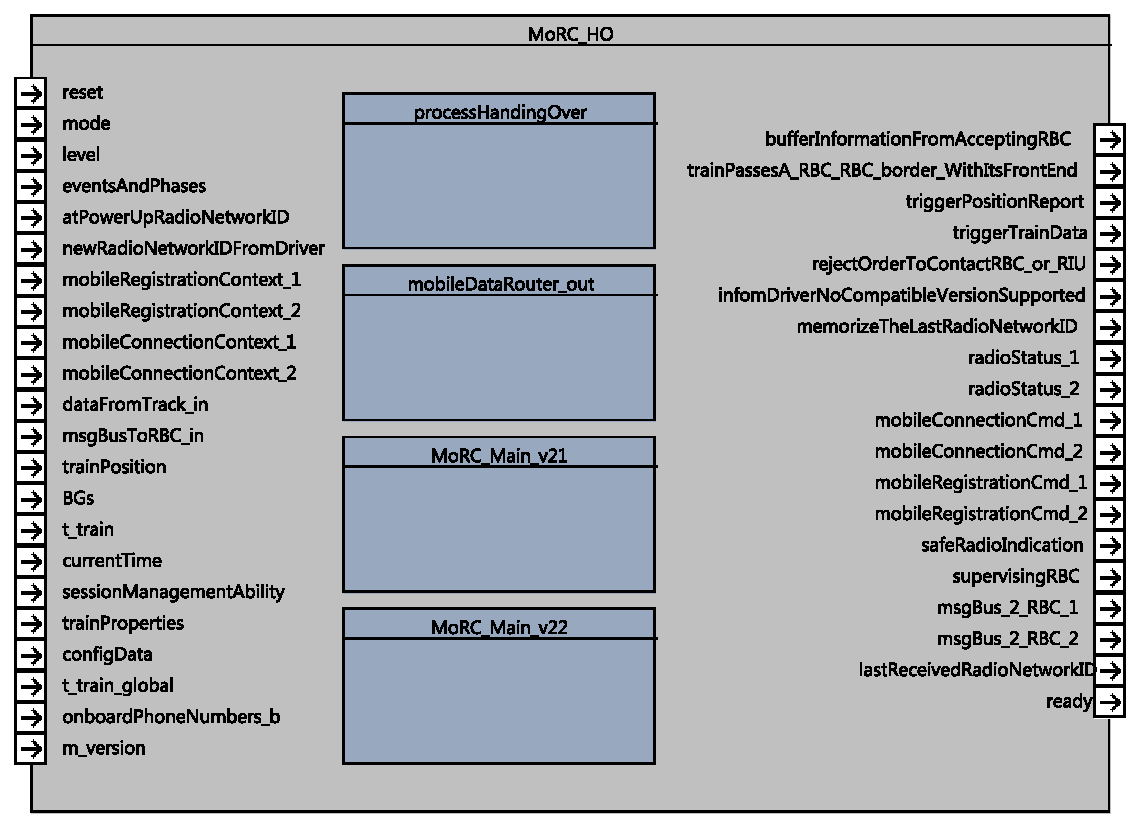
\includegraphics[width=0.9\linewidth]{images/F2_9_MoRC_HO.pdf}
\caption{Manage\_Radio\_Communication component SysML diagram}\label{f:manage_radio_communication_interface}
\end{figure}

\subsubsection{Inputs}\label{s:manage_radio_communication_inputs}

\paragraph{mode}

\begin{longtable}{p{.25\textwidth}p{.7\textwidth}}
\toprule
Input name				& mode \\
\midrule
Description				& Current onboard operating mode \\
\midrule
Source					& ??? \\ 
\midrule
Type					& M\_MODE \\
\midrule
Valid range of values	& Defined by M\_MODE enumerations \\
\midrule
Behaviour when value is at boundary	& n/a \\
\midrule
Behaviour for values out of valid range	& Code generation fails \\
\midrule
Behaviour when value is erroneous, absent or unwanted (i.e. spurious) & Misbehaviour \\
\bottomrule
\end{longtable}


\paragraph{[level]}

\begin{longtable}{p{.25\textwidth}p{.7\textwidth}}
\toprule
Input name				& level \\
\midrule
Description				& Current Operating Level \\
\midrule
Source					& ??? \\ 
\midrule
Type					& M\_LEVEL \\
\midrule
Valid range of values	& Defined by M\_LEVEL enumerations \\
\midrule
Behaviour when value is at boundary	& n/a \\
\midrule
Behaviour for values out of valid range	&  Code generation fails \\
\midrule
Behaviour when value is erroneous, absent or unwanted (i.e. spurious) & Misbehaviour \\
\bottomrule
\end{longtable}

\paragraph{eventsAndPhases}

\begin{longtable}{p{.25\textwidth}p{.7\textwidth}}
	\toprule
	Input name				& eventsAndPhases \\
	\midrule
	Description				& Collection of input events and OBU operating phases \\
	\midrule
	Source					& Collection of source components responsible for the information \\ 
	\midrule
	Type					& RCM\_Session\_Types\_Pkg::obuEventsAndPhases\_T \\
	\midrule
	Valid range of values	& n/a \\
	\midrule
	Behaviour when value is at boundary	& n/a \\
	\midrule
	Behaviour for values out of valid range	& Code generation fails \\
	\midrule
	Behaviour when value is erroneous, absent or unwanted (i.e. spurious) & Misbehaviour \\
	\bottomrule
\end{longtable}

\paragraph{atPowerUpRadioNetworkID}

\begin{longtable}{p{.25\textwidth}p{.7\textwidth}}
	\toprule
	Input name				& atPowerUpRadioNetworkID \\
	\midrule
	Description				& Radio network ID to be used at power up \\
	\midrule
	Source					& ??? \\ 
	\midrule
	Type					& Packet\_Types\_Pkg::P45\_RadioNetworkRegistration\_T \\
	\midrule
	Valid range of values	& Ref. to NID\_MN (Identity of Radio Network)  \\
	\midrule
	Behaviour when value is at boundary	& n/a \\
	\midrule
	Behaviour for values out of valid range	& OBU registers to unwanted radio network \\
	\midrule
	Behaviour when value is erroneous, absent or unwanted (i.e. spurious) & OBU registers to unwanted radio network  \\
	\bottomrule
\end{longtable}

\paragraph{newRadioNetworkIDFromDriver}

\begin{longtable}{p{.25\textwidth}p{.7\textwidth}}
	\toprule
	Input name				& newRadioNetworkIDFromDriver \\
	\midrule
	Description				& Radio network ID entered by the driver \\
	\midrule
	Source					& ??? \\ 
	\midrule
	Type					& Packet\_Types\_Pkg::P45\_RadioNetworkRegistration\_T \\
	\midrule
	Valid range of values	& Ref. to NID\_MN (Identity of Radio Network)  \\
	\midrule
	Behaviour when value is at boundary	& n/a \\
	\midrule
	Behaviour for values out of valid range	& OBU registers to unwanted radio network \\
	\midrule
	Behaviour when value is erroneous, absent or unwanted (i.e. spurious) & OBU registers to unwanted radio network  \\
	\bottomrule
\end{longtable}

\paragraph{mobileRegistrationContext\_1}

\begin{longtable}{p{.25\textwidth}p{.7\textwidth}}
	\toprule
	Input name				& mobileRegistrationContext\_1 \\
	\midrule
	Description				& Current registration status information from mobile modem 1 \\
	\midrule
	Source					& API \\ 
	\midrule
	Type					& RCM\_Types\_Pkg::mobileRegistrationContext\_T \\
	\midrule
	Valid range of values	& n/a \\
	\midrule
	Behaviour when value is at boundary	& n/a \\
	\midrule
	Behaviour for values out of valid range	& Misbehaviour \\
	\midrule
	Behaviour when value is erroneous, absent or unwanted (i.e. spurious) & Misbehaviour \\
	\bottomrule
\end{longtable}

\paragraph{mobileRegistrationContext\_2}

\begin{longtable}{p{.25\textwidth}p{.7\textwidth}}
	\toprule
	Input name				& mobileRegistrationContext\_2 \\
	\midrule
	Description				& Current registration status information from mobile modem 2 \\
	\midrule
	Source					& API \\ 
	\midrule
	Type					& RCM\_Types\_Pkg::mobileRegistrationContext\_T \\
	\midrule
	Valid range of values	& n/a \\
	\midrule
	Behaviour when value is at boundary	& n/a \\
	\midrule
	Behaviour for values out of valid range	& Misbehaviour \\
	\midrule
	Behaviour when value is erroneous, absent or unwanted (i.e. spurious) & Misbehaviour \\
	\bottomrule
\end{longtable}

\paragraph{mobileConnectionContext\_1}

\begin{longtable}{p{.25\textwidth}p{.7\textwidth}}
	\toprule
	Input name				& mobileConnectionContext\_2 \\
	\midrule
	Description				& Current connection status information from mobile modem 1 \\
	\midrule
	Source					& API \\ 
	\midrule
	Type					& RCM\_Types\_Pkg::mobileConnectionContext\_T \\
	\midrule
	Valid range of values	& n/a \\
	\midrule
	Behaviour when value is at boundary	& n/a \\
	\midrule
	Behaviour for values out of valid range	& Misbehaviour \\
	\midrule
	Behaviour when value is erroneous, absent or unwanted (i.e. spurious) & Misbehaviour \\
	\bottomrule
\end{longtable}

\paragraph{mobileConnectionContext\_2}

\begin{longtable}{p{.25\textwidth}p{.7\textwidth}}
	\toprule
	Input name				& mobileConnectionContext\_2 \\
	\midrule
	Description				& Current connection status information from mobile modem 2 \\
	\midrule
	Source					& API \\ 
	\midrule
	Type					& RCM\_Types\_Pkg::mobileConnectionContext\_T \\
	\midrule
	Valid range of values	& n/a \\
	\midrule
	Behaviour when value is at boundary	& n/a \\
	\midrule
	Behaviour for values out of valid range	& Misbehaviour \\
	\midrule
	Behaviour when value is erroneous, absent or unwanted (i.e. spurious) & Misbehaviour \\
	\bottomrule
\end{longtable}

\paragraph{dataFromTrack\_in}

\begin{longtable}{p{.25\textwidth}p{.7\textwidth}}
	\toprule
	Input name				& dataFromTrack\_in \\
	\midrule
	Description				& Messages received from track \\
	\midrule
	Source					&  Manage\_TrackSideInformation\_Integration \\ 
	\midrule
	Type					& RCM\_MsgTypes\_Pkg::msgFromTrack\_T \\
	\midrule
	Valid range of values	& n/a \\
	\midrule
	Behaviour when value is at boundary	& n/a \\
	\midrule
	Behaviour for values out of valid range	& Misbehaviour \\
	\midrule
	Behaviour when value is erroneous, absent or unwanted (i.e. spurious) & Misbehaviour \\
	\bottomrule
\end{longtable}

\paragraph{dataToRBC\_in}

\begin{longtable}{p{.25\textwidth}p{.7\textwidth}}
	\toprule
	Input name				& dataToRBC\_in \\
	\midrule
	Description				& Messages to be routed to the supervising RBC \\
	\midrule
	Source					& All components transmitting messages to the RBC \\ 
	\midrule
	Type					& RCM\_MsgTypes\_Pkg::msgToTrack\_T \\
	\midrule
	Valid range of values	& n/a \\
	\midrule
	Behaviour when value is at boundary	& n/a \\
	\midrule
	Behaviour for values out of valid range	& Confused RBC communication\\
	\midrule
	Behaviour when value is erroneous, absent or unwanted (i.e. spurious) & Confused RBC communication \\
	\bottomrule
\end{longtable}

\paragraph{positionReport\_in}

\begin{longtable}{p{.25\textwidth}p{.7\textwidth}}
	\toprule
	Input name				& positionReport\_in \\
	\midrule
	Description				& Current positon report to be transmitted to the handing over and/or accepting RBC under control of \emph{MoRC\_HO}\\
	\midrule
	Source					& providePositionReport \\ 
	\midrule
	Type					& RCM\_MsgTypes\_Pkg::msgToTrack\_T \\
	\midrule
	Valid range of values	& n/a \\
	\midrule
	Behaviour when value is at boundary	& n/a \\
	\midrule
	Behaviour for values out of valid range	& RBC receives faulty position report \\
	\midrule
	Behaviour when value is erroneous, absent or unwanted (i.e. spurious) & RBC receives faulty position report \\
	\bottomrule
\end{longtable}

\paragraph{trainData\_in}

\begin{longtable}{p{.25\textwidth}p{.7\textwidth}}
	\toprule
	Input name				& trainData\_in \\
	\midrule
	Description				& Validated train data (packet 11) to be transmitted to the handing over and/or accepting RBC under control of \emph{MoRC\_HO} \\
	\midrule
	Source					& ??? \\ 
	\midrule
	Type					& RCM\_MsgTypes\_Pkg::msgToTrack\_T \\
	\midrule
	Valid range of values	& n/a \\
	\midrule
	Behaviour when value is at boundary	& n/a \\
	\midrule
	Behaviour for values out of valid range	& RBC receives faulty train data \\
	\midrule
	Behaviour when value is erroneous, absent or unwanted (i.e. spurious) & RBC receives faulty train data \\
	\bottomrule
\end{longtable}

\paragraph{trainPosition}

\begin{longtable}{p{.25\textwidth}p{.7\textwidth}}
	\toprule
	Input name				& trainPosition \\
	\midrule
	Description				& Current train position \\
	\midrule
	Source					& calculateTrainPosition \\ 
	\midrule
	Type					& TrainPosition\_Types\_Pck::trainPosition\_T \\
	\midrule
	Valid range of values	& n/a \\
	\midrule
	Behaviour when value is at boundary	& n/a \\
	\midrule
	Behaviour for values out of valid range	& RBC handover is performed at an unwanted location \\
	\midrule
	Behaviour when value is erroneous, absent or unwanted (i.e. spurious) & RBC handover is performed at an unwanted location \\
	\bottomrule
\end{longtable}

\paragraph{BGs}

\begin{longtable}{p{.25\textwidth}p{.7\textwidth}}
	\toprule
	Input name				& BGs \\
	\midrule
	Description				& Collection of currently known balise groups \\
	\midrule
	Source					& calculateTrainPosition \\ 
	\midrule
	Type					& TrainPosition\_Types\_Pck::positionedBGs\_T \\
	\midrule
	Valid range of values	& n/a \\
	\midrule
	Behaviour when value is at boundary	& n/a \\
	\midrule
	Behaviour for values out of valid range	& RBC handover is performed at an unwanted location \\
	\midrule
	Behaviour when value is erroneous, absent or unwanted (i.e. spurious) & RBC handover is performed at an unwanted location \\
	\bottomrule
\end{longtable}

\paragraph{t\_train}

\begin{longtable}{p{.25\textwidth}p{.7\textwidth}}
	\toprule
	Input name				& t\_train \\
	\midrule
	Description				& Time, according to trainborne clock, at which messages are to be sent \\
	\midrule
	Source					& ??? \\ 
	\midrule
	Type					& T\_TRAIN \\
	\midrule
	Valid range of values	& Refer to Subset 016-7. \\
	\midrule
	Behaviour when value is at boundary	& n/a \\
	\midrule
	Behaviour for values out of valid range	& Faulty time information in messages sent to the RBC \\
	\midrule
	Behaviour when value is erroneous, absent or unwanted (i.e. spurious) & Faulty time information in messages sent to the RBC \\
	\bottomrule
\end{longtable}

\paragraph{reset}

\begin{longtable}{p{.25\textwidth}p{.7\textwidth}}
	\toprule
	Input name				& reset \\
	\midrule
	Description				& Initializes the component and deletes the internal storage \\
	\midrule
	Source					& The OBUs system start controller \\ 
	\midrule
	Type					& bool \\
	\midrule
	Valid range of values	& true | false \\
	\midrule
	Behaviour when value is at boundary	& n/a \\
	\midrule
	Behaviour for values out of valid range	& Code generation fails \\
	\midrule
	Behaviour when value is erroneous, absent or unwanted (i.e. spurious) & Misbehaviour \\
	\bottomrule
\end{longtable}

\paragraph{sessionManagementAbility}

\begin{longtable}{p{.25\textwidth}p{.7\textwidth}}
	\toprule
	Input name				& sessionManagementAbility \\
	\midrule
	Description				& Configurable ability to manage one or two sessions and mobile modems onboard \\
	\midrule
	Source					& The OBUs configuration manager \\ 
	\midrule
	Type					& Handover\_Pkg::abilityToHandleCommunicationSessions \\
	\midrule
	Valid range of values	& isAbleToManageOneSession | isAbleToManageTwoSessions \\
	\midrule
	Behaviour when value is at boundary	& n/a \\
	\midrule
	Behaviour for values out of valid range	& Code generation fails \\
	\midrule
	Behaviour when value is erroneous, absent or unwanted (i.e. spurious) & Misbehaviour \\
	\bottomrule
\end{longtable}

\paragraph{trainProperties}

\begin{longtable}{p{.25\textwidth}p{.7\textwidth}}
	\toprule
	Input name				& trainProperties \\
	\midrule
	Description				& Train parameters used to calculate the handover location and to generate messages to the RBC \\
	\midrule
	Source					& The OBUs configuration manager \\ 
	\midrule
	Type					& TrainPosition\_Types\_Pck::trainProperties\_T \\
	\midrule
	Valid range of values	& n/a \\
	\midrule
	Behaviour when value is at boundary	& n/a \\
	\midrule
	Behaviour for values out of valid range	& Faulty parametrization \\
	\midrule
	Behaviour when value is erroneous, absent or unwanted (i.e. spurious) & Misbehaviour \\
	\bottomrule
\end{longtable}

\paragraph{configData}

\begin{longtable}{p{.25\textwidth}p{.7\textwidth}}
	\toprule
	Input name				& configData \\
	\midrule
	Description				& Session management configuration parameters \\
	\midrule
	Source					& The OBUs configuration manager \\ 
	\midrule
	Type					& RCM\_Session\_Types\_Pkg::morc\_configData\_T \\
	\midrule
	Valid range of values	& n/a \\
	\midrule
	Behaviour when value is at boundary	& n/a \\
	\midrule
	Behaviour for values out of valid range	& Misbehaviour \\
	\midrule
	Behaviour when value is erroneous, absent or unwanted (i.e. spurious) & Misbehaviour \\
	\bottomrule
\end{longtable}


\subsubsection{Outputs}\label{s:manage_radio_communication_outputs}

\paragraph{radioStatus\_1}

\begin{longtable}{p{.25\textwidth}p{.7\textwidth}}
\toprule
Output name				& radioStatus\_1 \\
\midrule
Description				& Radio registration, connection and session status for radio link 1 \\
\midrule
Destination				& All components which need to know the radio status \\ 
\midrule
Type					& RCM\_Session\_Types\_Pkg::morcStatus\_T \\
\midrule
Valid range of values	& n/a \\
\midrule
Behaviour when value is at boundary	& n/a \\
\midrule
Behaviour for values out of valid range	& n/a \\
\midrule
Behaviour when value is erroneous, absent or unwanted (i.e. spurious) & n/a \\
\bottomrule
\end{longtable}

\paragraph{radioStatus\_2}

\begin{longtable}{p{.25\textwidth}p{.7\textwidth}}
	\toprule
	Output name				& radioStatus\_2 \\
	\midrule
	Description				& Radio registration, connection and session status for radio link 2 \\
	\midrule
	Destination				& All components which need to know the radio status \\ 
	\midrule
	Type					& RCM\_Session\_Types\_Pkg::morcStatus\_T \\
	\midrule
	Valid range of values	& n/a \\
	\midrule
	Behaviour when value is at boundary	& n/a \\
	\midrule
	Behaviour for values out of valid range	& n/a \\
	\midrule
	Behaviour when value is erroneous, absent or unwanted (i.e. spurious) & n/a \\
	\bottomrule
\end{longtable}

\paragraph{mobileConnectionCmd\_1}

\begin{longtable}{p{.25\textwidth}p{.7\textwidth}}
	\toprule
	Output name				& mobileConnectionCmd\_1 \\
	\midrule
	Description				& Commands to mobile 1 for radio connection control  \\
	\midrule
	Destination				& API to radio mobile 1 \\ 
	\midrule
	Type					& RCM\_Types\_Pkg::mobileConnectionCmd\_T \\
	\midrule
	Valid range of values	& n/a \\
	\midrule
	Behaviour when value is at boundary	& n/a \\
	\midrule
	Behaviour for values out of valid range	& n/a \\
	\midrule
	Behaviour when value is erroneous, absent or unwanted (i.e. spurious) & n/a \\
	\bottomrule
\end{longtable}

\paragraph{mobileConnectionCmd\_2}

\begin{longtable}{p{.25\textwidth}p{.7\textwidth}}
	\toprule
	Output name				& mobileConnectionCmd\_2 \\
	\midrule
	Description				& Commands to mobile 2 for radio connection control  \\
	\midrule
	Destination				& API to radio mobile 2 \\ 
	\midrule
	Type					& RCM\_Types\_Pkg::mobileConnectionCmd\_T \\
	\midrule
	Valid range of values	& n/a \\
	\midrule
	Behaviour when value is at boundary	& n/a \\
	\midrule
	Behaviour for values out of valid range	& n/a \\
	\midrule
	Behaviour when value is erroneous, absent or unwanted (i.e. spurious) & n/a \\
	\bottomrule
\end{longtable}

\paragraph{mobileRegistrationCmd\_1}

\begin{longtable}{p{.25\textwidth}p{.7\textwidth}}
	\toprule
	Output name				& mobileRegistrationCmd\_1 \\
	\midrule
	Description				& Commands to mobile 1 for radio registration control  \\
	\midrule
	Destination				& API to radio mobile 1 \\ 
	\midrule
	Type					& RCM\_Types\_Pkg::mobileRegistrationCmd\_T \\
	\midrule
	Valid range of values	& n/a \\
	\midrule
	Behaviour when value is at boundary	& n/a \\
	\midrule
	Behaviour for values out of valid range	& n/a \\
	\midrule
	Behaviour when value is erroneous, absent or unwanted (i.e. spurious) & n/a \\
	\bottomrule
\end{longtable}

\paragraph{mobileRegistrationCmd\_2}

\begin{longtable}{p{.25\textwidth}p{.7\textwidth}}
	\toprule
	Output name				& mobileRegistrationCmd\_2 \\
	\midrule
	Description				& Commands to mobile 2 for radio registration control  \\
	\midrule
	Destination				& API to radio mobile 2 \\ 
	\midrule
	Type					& RCM\_Types\_Pkg::mobileRegistrationCmd\_T \\
	\midrule
	Valid range of values	& n/a \\
	\midrule
	Behaviour when value is at boundary	& n/a \\
	\midrule
	Behaviour for values out of valid range	& n/a \\
	\midrule
	Behaviour when value is erroneous, absent or unwanted (i.e. spurious) & n/a \\
	\bottomrule
\end{longtable}

\paragraph{safeRadioIndication}

\begin{longtable}{p{.25\textwidth}p{.7\textwidth}}
	\toprule
	Output name				& safeRadioIndication \\
	\midrule
	Description				& Safe radio indication for DMI  \\
	\midrule
	Destination				& DIM via DMI interface \\ 
	\midrule
	Type					& RCM\_Session\_Types\_Pkg::safeRadioConnectionIndication\_T \\
	\midrule
	Valid range of values	& srci\_noConnection | srci\_connectionLost\_setupFailed | srci\_connectionUp \\
	\midrule
	Behaviour when value is at boundary	& n/a \\
	\midrule
	Behaviour for values out of valid range	& n/a \\
	\midrule
	Behaviour when value is erroneous, absent or unwanted (i.e. spurious) & n/a \\
	\bottomrule
\end{longtable}

\paragraph{supervisingRBC}

\begin{longtable}{p{.25\textwidth}p{.7\textwidth}}
	\toprule
	Output name				& supervisingRBC \\
	\midrule
	Description				& Designates the current supervising RBC for the InformationFilter to support input message filtering and buffering there \\
	\midrule
	Destination				& InformationFilter \\ 
	\midrule
	Type					& Handover\_Pkg::connection\_ids\_T \\
	\midrule
	Valid range of values	& n/a \\
	\midrule
	Behaviour when value is at boundary	& n/a \\
	\midrule
	Behaviour for values out of valid range	& n/a \\
	\midrule
	Behaviour when value is erroneous, absent or unwanted (i.e. spurious) & n/a \\
	\bottomrule
\end{longtable}

\paragraph{bufferInformationFromAcceptingRBC}

\begin{longtable}{p{.25\textwidth}p{.7\textwidth}}
	\toprule
	Output name				& bufferInformationFromAcceptingRBC \\
	\midrule
	Description				& Informs the InfomationFilter to buffer messages received from the accepting RBC \\
	\midrule
	Destination				& InformationFilter \\ 
	\midrule
	Type					& bool \\
	\midrule
	Valid range of values	& true | false \\
	\midrule
	Behaviour when value is at boundary	& n/a \\
	\midrule
	Behaviour for values out of valid range	& Code generation fails \\
	\midrule
	Behaviour when value is erroneous, absent or unwanted (i.e. spurious) & Misbehaviour \\
	\bottomrule
\end{longtable}

\paragraph{trainPassesA\_RBC\_RBC\_border\_WithItsFrontEnd}

\begin{longtable}{p{.25\textwidth}p{.7\textwidth}}
	\toprule
	Output name				& trainPassesA\_RBC\_RBC\_border\_WithItsFrontEnd \\
	\midrule
	Description				& Indicates that the train front passes a RBC/RBC border. \\
	\midrule
	Destination				& To whom it may concern \\ 
	\midrule
	Type					& bool \\
	\midrule
	Valid range of values	& true | false \\
	\midrule
	Behaviour when value is at boundary	& n/a \\
	\midrule
	Behaviour for values out of valid range	& Code generation fails \\
	\midrule
	Behaviour when value is erroneous, absent or unwanted (i.e. spurious) & Misbehaviour \\
	\bottomrule
\end{longtable}

\paragraph{msgToRBC\_1}

\begin{longtable}{p{.25\textwidth}p{.7\textwidth}}
	\toprule
	Output name				& msgToRBC\_1 \\
	\midrule
	Description				& Radio message to be transmitted to RBC via mobile modem 1, if session established. \\
	\midrule
	Destination				& API: interface to mobile modem 1 \\ 
	\midrule
	Type					& RCM\_MsgTypes\_Pkg::msgToTrack\_T \\
	\midrule
	Valid range of values	& n/a \\
	\midrule
	Behaviour when value is at boundary	& n/a \\
	\midrule
	Behaviour for values out of valid range	& n/a \\
	\midrule
	Behaviour when value is erroneous, absent or unwanted (i.e. spurious) & n/a \\
	\bottomrule
\end{longtable}

\paragraph{msgToRBC\_2}

\begin{longtable}{p{.25\textwidth}p{.7\textwidth}}
	\toprule
	Output name				& msgToRBC\_2 \\
	\midrule
	Description				& Radio message to be transmitted to RBC via mobile modem 2, if session established. \\
	\midrule
	Destination				& API: interface to mobile modem 2 \\ 
	\midrule
	Type					& RCM\_MsgTypes\_Pkg::msgToTrack\_T \\
	\midrule
	Valid range of values	& n/a \\
	\midrule
	Behaviour when value is at boundary	& n/a \\
	\midrule
	Behaviour for values out of valid range	& n/a \\
	\midrule
	Behaviour when value is erroneous, absent or unwanted (i.e. spurious) & n/a \\
	\bottomrule
\end{longtable}

\paragraph{triggerPositionReport}

\begin{longtable}{p{.25\textwidth}p{.7\textwidth}}
	\toprule
	Output name				& triggerPositionReport \\
	\midrule
	Description				& Triggers the providePositionReport function to provide a position report at positionReport\_in input. \\
	\midrule
	Destination				& providePositionReport \\ 
	\midrule
	Type					& bool \\
	\midrule
	Valid range of values	& true | false \\
	\midrule
	Behaviour when value is at boundary	& n/a \\
	\midrule
	Behaviour for values out of valid range	& Code generation fails \\
	\midrule
	Behaviour when value is erroneous, absent or unwanted (i.e. spurious) & Causes a mistimed position report  \\
	\bottomrule
\end{longtable}


\paragraph{triggerTrainData}

\begin{longtable}{p{.25\textwidth}p{.7\textwidth}}
	\toprule
	Output name				& triggerTrainData \\
	\midrule
	Description				& Triggers the provideTrainData function to provide a train data set (packet 11) at trainData\_in input \\
	\midrule
	Destination				& provideTrainData ??? \\ 
	\midrule
	Type					& bool \\
	\midrule
	Valid range of values	& true | false \\
	\midrule
	Behaviour when value is at boundary	& n/a \\
	\midrule
	Behaviour for values out of valid range	& Code generation fails \\
	\midrule
	Behaviour when value is erroneous, absent or unwanted (i.e. spurious) & Causes a mistimed train data set transmission to the RBC \\
	\bottomrule
\end{longtable}

\paragraph{rejectOrderToContactRBC\_or\_RIU}

\begin{longtable}{p{.25\textwidth}p{.7\textwidth}}
	\toprule
	Output name				& rejectOrderToContactRBC\_or\_RIU \\
	\midrule
	Description				& Informs the OBU that the order to contact an RBC has to be rejected \\
	\midrule
	Destination				& ??? \\ 
	\midrule
	Type					& bool \\
	\midrule
	Valid range of values	& true | false \\
	\midrule
	Behaviour when value is at boundary	& n/a \\
	\midrule
	Behaviour for values out of valid range	& Code generation fails \\
	\midrule
	Behaviour when value is erroneous, absent or unwanted (i.e. spurious) & n/a \\
	\bottomrule
\end{longtable}

\paragraph{infomDriverNoCompatibleVersionSupported}

\begin{longtable}{p{.25\textwidth}p{.7\textwidth}}
	\toprule
	Output name				& infomDriverNoCompatibleVersionSupported \\
	\midrule
	Description				& Informs the driver that no compatible version is. supported \\
	\midrule
	Destination				& DMI via DMI interface and API \\ 
	\midrule
	Type					& bool \\
	\midrule
	Valid range of values	& true | false \\
	\midrule
	Behaviour when value is at boundary	& n/a \\
	\midrule
	Behaviour for values out of valid range	& Code generation fails \\
	\midrule
	Behaviour when value is erroneous, absent or unwanted (i.e. spurious) & Misinformed train driver \\
	\bottomrule
\end{longtable}

\paragraph{memorizeTheLastRadioNetworkID}

\begin{longtable}{p{.25\textwidth}p{.7\textwidth}}
	\toprule
	Output name				& memorizeTheLastRadioNetworkID \\
	\midrule
	Description				& Triggers the storage of the last radio network ID. \\
	\midrule
	Destination				& External storage via API \\ 
	\midrule
	Type					& bool \\
	\midrule
	Valid range of values	& true | false \\
	\midrule
	Behaviour when value is at boundary	& n/a \\
	\midrule
	Behaviour for values out of valid range	& Code generation fails \\
	\midrule
	Behaviour when value is erroneous, absent or unwanted (i.e. spurious) & Corrupted stored last radio network ID \\
	\bottomrule
\end{longtable}


\paragraph{lastReceivedRadioNetworkID}

\begin{longtable}{p{.25\textwidth}p{.7\textwidth}}
	\toprule
	Output name				& lastReceivedRadioNetworkID \\
	\midrule
	Description				& Provides the last received radio network ID. \\
	\midrule
	Destination				& External storage via API \\ 
	\midrule
	Type					& Packet\_Types\_Pkg::P45\_RadioNetworkRegistration\_T \\
	\midrule
	Valid range of values	& Refer to subset 026-7, packet 45 \\
	\midrule
	Behaviour when value is at boundary	& n/a \\
	\midrule
	Behaviour for values out of valid range	& Code generation fails \\
	\midrule
	Behaviour when value is erroneous, absent or unwanted (i.e. spurious) & Corrupted stored last radio network ID \\
	\bottomrule
\end{longtable}

\paragraph{ready}

\begin{longtable}{p{.25\textwidth}p{.7\textwidth}}
	\toprule
	Output name				& ready \\
	\midrule
	Description				& When false, indicates that MoRC\_HO has not finished the current operation and needs at least one more clock before the next input event can be consumed. \\
	\midrule
	Destination				& All components providing inputs for MoRC\_HO \\ 
	\midrule
	Type					& bool \\
	\midrule
	Valid range of values	& true | false \\
	\midrule
	Behaviour when value is at boundary	& n/a \\
	\midrule
	Behaviour for values out of valid range	& n/a \\
	\midrule
	Behaviour when value is erroneous, absent or unwanted (i.e. spurious) & Misbehaviour \\
	\bottomrule
\end{longtable}



\subsection{Subcomponents}\label{s:manage_radio_communication_subcomponents}

\subsubsection{RBC\_Handover}
%set the master document for easy compilation
%!TEX root = ../D3_5_3.tex

\paragraph{Component Requirements}

\begin{longtable}{p{.25\textwidth}p{.7\textwidth}}
\toprule
Component name			& processHandingOver \\
\midrule
Link to SCADE model		& {\footnotesize \url{https://github.com/openETCS/modeling/tree/master/model/Scade/System/ObuFunctions/Radio/Handover/RBC_Handover}} \\
\midrule
SCADE designer			& Uwe Steinke, Siemens \\
\midrule
Description				& 
The function \emph{processHandingOver} implements the process of handing over the OBU from one RBC to a subsequent RBC. This process is based upon orders received from balise and radio. 
\newline
\newline
\emph{processHandingOver} terminates the radio session with the current - the handing over - RBC and establishes a session with the new - the accepting - RBC. Dependent on the availability of one or two mobile modems onboard, \emph{processHandingOver} is able to manage two sessions in parallel or subsequently. For this, it steers two instances of MoRC\_Main\_v2. \newline

\emph{processHandingOver} controls the switchover of the OBUs output data stream to track from the handing over RBC to the accepting RBC and provides the InformationFilter with the supervising RBC information for message buffering and filtering. 

It in addition, \emph{processHandingOver} monitors the current train position and executes the handover, when the train front passes the apppropriate location. 

\\
\midrule
Input documents	& 
Subset-026, Chapter 3.15 \newline
Subset-026, Chapter 5.15 \\
\midrule
Safety integrity level		& 4 \\
\midrule
Time constraints		& Implements several time delays, therefore appropriate clocking required \\
\midrule
API requirements 		& n/a \\
\bottomrule
\end{longtable}


\paragraph{Interface}

For an overview of the interface of this internal component we refer to the SCADE model (cf.~link above) respectively the SCADE generated documentation.

\subsubsection{Management\_of\_Radio\_Communication}
%set the master document for easy compilation
%!TEX root = ../D3_5_3.tex

\paragraph{Component Requirements}

\begin{longtable}{p{.25\textwidth}p{.7\textwidth}}
\toprule
Component name			& MoRC\_Main\_v2 (Management\_of\_Radio\_Communication) \\
\midrule
Link to SCADE model		& {\footnotesize \url{https://github.com/openETCS/modeling/tree/master/model/Scade/System/ObuFunctions/Radio/MoRC}} \\
\midrule
SCADE designer			& Uwe Steinke, Siemens \\
\midrule
Description				& 
The function \emph{MoRC\_Main\_v2} implements the session states establishing, maintaining and terminating as described in Subset-026, chap. 3.5. A SCADE state machine reflects this state model  accurately. Within each of the states, the activities needed as long as the state is active, are performed. \newline

\emph{MoRC\_Main\_v2} is related to exactly one of the radio mobile modems onboard, monitors its status and controls the processes of registration to the radio network, connecting to one RBC and establishing a radio session with the RBC. \emph{MoRC\_Main\_v2} communicates with its mobile modem directly via the API.  \newline

As the OBU is required to manage up to two RBCs,  two instances of \emph{MoRC\_Main\_v2} are used.  \newline

In addition, \emph{MoRC\_Main\_v2} generates the radio connection indication for the driver.

\\
\midrule
Input documents	& 
Subset-026, Chapter 3.5 \\
\midrule
Safety integrity level		& 4 \\
\midrule
Time constraints		& Implements several time delays, therefore appropriate clocking required \\
\midrule
API requirements 		& Interfaces to the OBUs mobile modem hardware via API \\
\bottomrule
\end{longtable}


\paragraph{Interface}

For an overview of the interface of this internal component we refer to the SCADE model (cf.~link above) respectively the SCADE generated documentation.

\subsubsection{mobileDataRouter}
%set the master document for easy compilation
%!TEX root = ../D3_5_3.tex

\paragraph{Component Requirements}

\begin{longtable}{p{.25\textwidth}p{.7\textwidth}}
\toprule
Component name			& mobileDataRouter\_out \\
\midrule
Link to SCADE model		& {\footnotesize \url{https://github.com/openETCS/modeling/tree/master/model/Scade/System/ObuFunctions/Radio/Handover/RBC_Handover}} \\
\midrule
SCADE designer			& Uwe Steinke, Siemens \\
\midrule
Description				& 
The function \emph{mobileDataRouter\_out} represents the change-over switch commutating the OBUs output message data stream from the handing over RBC to the accepting RBC. It is controlled by the processHandingOver subcomponent.

\\
\midrule
Input documents	& 
Subset-026, Chapter 3.15 \newline
Subset-026, Chapter 5.15 \\
\midrule
Safety integrity level		& 4 \\
\midrule
Time constraints		& n/a \\
\midrule
API requirements 		& n/a \\
\bottomrule
\end{longtable}


\paragraph{Interface}

For an overview of the interface of this internal component we refer to the SCADE model (cf.~link above) respectively the SCADE generated documentation.
